\section{The mechanics: a Monte Carlo simulation of the model}
\label{sec:mc}

Before I trusted my own derivation enough to run it on a real bank, I wanted to prove it to myself the hard way. The closed-form $\PD=\Ncdf(-\DD)$ is a statement about a random variable. A \emph{Monte Carlo simulation} tests such a statement by brute force: generate many random futures, count how often the event occurs, and see whether the count matches the formula. This section is me checking my own homework before I let the model anywhere near Yes Bank's actual share price.

\begin{defbox}{Monte Carlo simulation}
Draw a large number of random scenarios from the model, record for each whether default occurred, and take the fraction of scenarios with default as the estimated probability. By the law of large numbers the estimate converges to the true probability, with a standard error of about $\sqrt{p(1-p)/n}$ for $n$ scenarios.
\end{defbox}

\paragraph{Algorithm.} (1) Fix $V_0$, $D$, $\mu$, $\sigma$, $T$. (2) For each scenario draw $Z\sim\text{N}(0,1)$ and compute $V_T$ from equation~\eqref{eq:gbmsol}. (3) Count the fraction of scenarios with $V_T<D$. (4) Compare with $\Ncdf(-\DD)$. A second version simulates the whole path in daily steps and counts a default if the path ever touches $D$ (a \emph{barrier} or first-passage variant, following Black and Cox \cite{blackcox1976}). That variant gives a higher probability because a path can dip below $D$ and recover before $T$; Merton's original model counts default only at $T$.

\begin{figure}[H]\centering
\includegraphics[width=0.62\textwidth]{figs/gbm_paths.png}\hfill
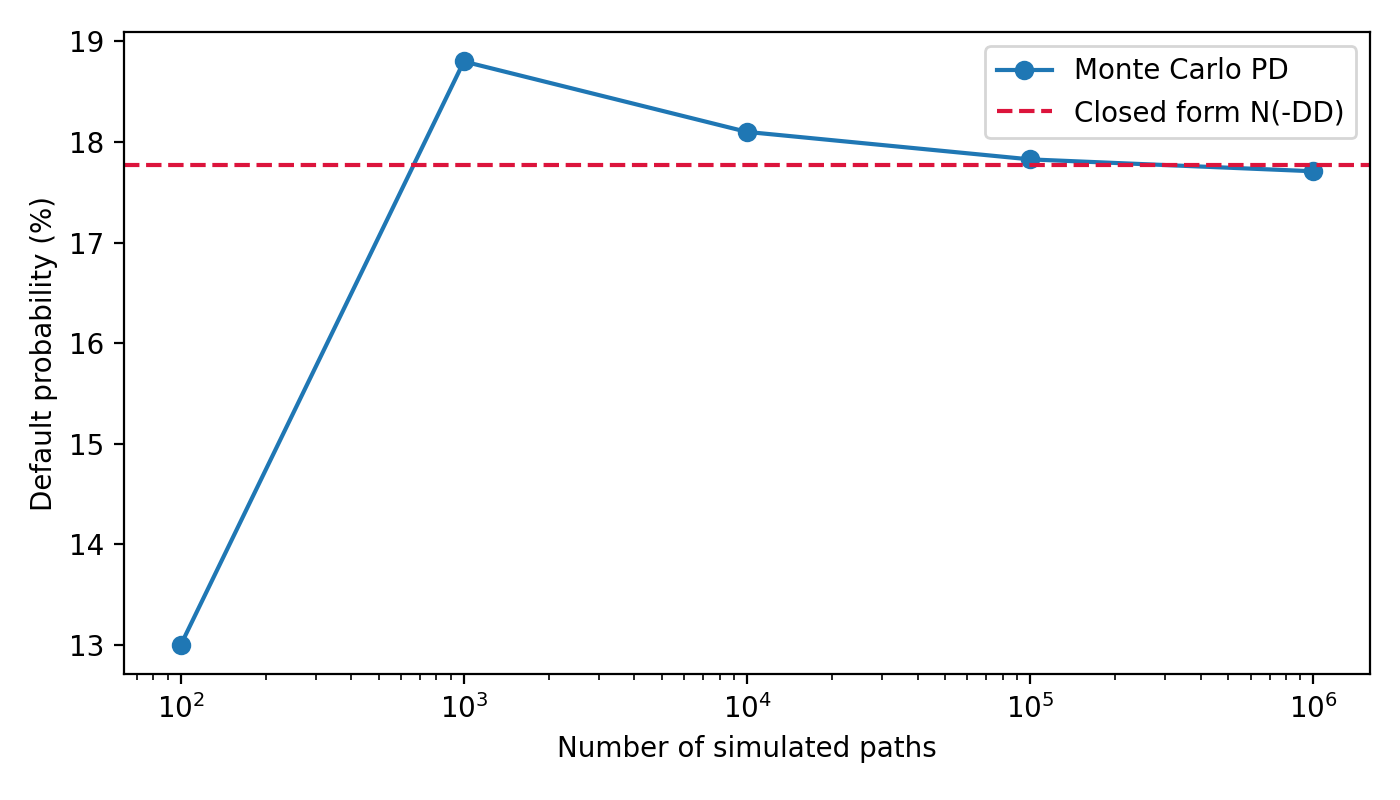
\includegraphics[width=0.36\textwidth]{mc_convergence.png}
\caption{Left: 60 simulated GBM asset paths for the illustrative firm; red paths end below the default point $D=100$. Right: the Monte Carlo default probability converges to the closed-form value as the number of paths grows.}
\end{figure}

\lstinputlisting[caption={Monte Carlo check of the Merton default probability (file \texttt{merton\_monte\_carlo.py}). Run in VS Code after \texttt{pip install numpy scipy matplotlib}.},label={lst:mc}]{merton_monte_carlo.py}

\paragraph{Output of the listing.}
\begin{center}\small
\begin{tabular}{rrrr}\toprule
\textbf{Paths} & \textbf{MC PD} & \textbf{95\% CI $\pm$} & \textbf{Abs.\ error}\\\midrule
100 & 13.00\% & 6.59\% & 4.77\%\\
1,000 & 18.80\% & 2.42\% & 1.03\%\\
10,000 & 18.10\% & 0.75\% & 0.33\%\\
100,000 & 17.83\% & 0.24\% & 0.06\%\\
1,000,000 & 17.71\% & 0.07\% & 0.06\%\\\midrule
\multicolumn{4}{c}{Closed form $\Ncdf(-\DD)$ with $\DD=0.9243$: \textbf{17.77\%}. Barrier variant (100k paths): 37.7\%.}\\\bottomrule
\end{tabular}
\end{center}
The simulated PD converges to the formula, and the errors sit inside the confidence interval. (Exact figures for small $n$ depend on the random seed.)

\section{The case: Yes Bank, 2018--2020}
\label{sec:case}

This is the part of the project where I stopped working with an illustrative firm and started working with a real one. Everything from here on uses Yes Bank's actual traded price, Yes Bank's actual published balance sheets, and the actual dated public record of what the rating agencies and the RBI did. I went back after my first draft and verified every date I was unsure of against a primary source — a regulatory filing, a press release, or a SEBI order — rather than leaving them as things I could not check. I'll flag the handful of places where I still could not get a primary source, but the list is much shorter now than when I started.

\subsection{Timeline from the public record, verified}
Sources are numbered in the bibliography. A date I verified against a company filing, an agency's own press release, or a regulator's order is given without a qualifier. A date that still rests only on secondary news reporting is marked so, honestly, rather than dressed up as something I confirmed.

\begingroup\small
\renewcommand{\arraystretch}{1.15}
\begin{longtable}{@{}>{\raggedright\arraybackslash}p{2.5cm}p{11.1cm}@{}}
\toprule\textbf{Date} & \textbf{Event}\\\midrule\endhead
12 May 2017 & Annual report discloses RBI-assessed FY16 gross NPAs of Rs 4,925.68 crore against Rs 748.98 crore reported: a divergence of Rs 4,176.70 crore \cite{bsDivFY16}.\\
5 Jul 2018 & CARE upgrades senior and Tier II debt to AAA from AA+ --- the first AAA any agency had given Yes Bank, and only the fourth private bank in India (after HDFC, ICICI and Kotak) to hold it \cite{bsCareWatch,sebiCareOrder}. Share price: Rs 349.\\
20 Aug 2018 & Share price peaks (closing high Rs 394 in our data; intraday high Rs 404).\\
17 Sep 2018 & \textbf{Verified.} The RBI's letter curtailing Rana Kapoor's term as MD \& CEO to 31 January 2019 is dated this day. The bank received it the same day, but did not disclose it to the exchanges until the evening of 19 September \cite{bsSep19disc}.\\
19--21 Sep 2018 & The disclosure becomes public on 19 September (a Wednesday); the stock falls across the next two trading sessions, with the sharpest single-day fall (around 29--34\%, depending on the exchange and the moment measured) on 21 September \cite{bsSep21fall}. My own price series has no entry for 20 September.\\
1 Oct 2018 & \textbf{Verified.} CARE places the AAA rating on credit watch with developing implications, citing the RBI's communication on Kapoor's tenure \cite{bsCareOct1}.\\
17 Nov 2018 & ICRA places Yes Bank on watch with negative implications \cite{bsIcraWatch}.\\
27 Nov 2018 & Moody's cuts the foreign-currency issuer rating to Ba1 from Baa3 \cite{bsNov28}.\\
28 Nov 2018 & ICRA downgrades senior debt to AA (from AA+) and subordinated to AA$-$ (from AA); CARE downgrades senior to AA+ (from AAA) and subordinated to AA (from AA+) \cite{bsNov28}.\\
24 Jan 2019 & Q3 FY19 results; RBI approves Ravneet Gill as MD \& CEO, to join on or before 1 Mar 2019 \cite{bsQ3FY19}.\\
13 Feb 2019 & Bank states that the RBI found no divergence for FY18; the same report recalls the FY17 divergence (RBI-assessed gross NPAs Rs 8,373.8 crore against Rs 2,018 crore reported) \cite{bsDivFY18}.\\
30 Apr 2019 & Share falls about 29\% on the first session after the first-ever quarterly loss (Rs 1,506 crore in Q4 FY19) \cite{bsFall19}.\\
3 May 2019 & ICRA downgrades Tier I bonds to A (from AA$-$) and Tier II to AA$-$ (from AA), outlook negative \cite{bsIcraMay19,icraJul19}.\\
8 May 2019 & \textbf{Verified.} India Ratings cuts the long-term issuer rating to IND~AA$-$ from IND~AA+, negative outlook; filed late evening, reported the next morning \cite{bsIndraMay19}.\\
24 Jul 2019 & ICRA downgrades a Rs 32,911.7 crore bond programme (one notch on Rs 22,111.7 crore; two notches on Rs 10,800 crore of AT-1) \cite{icraJul19,bsIcraJul19}.\\
15 Aug 2019 (approx.) & QIP (a share sale to institutional investors) raises Rs 1,930 crore \cite{ycQ2}.\\
31 Aug 2019 & India Ratings downgrades further, to IND~A+ from IND~AA$-$, negative outlook --- citing slower-than-expected resolution of stressed assets and a smaller-than-hoped capital raise even after the QIP \cite{bsIndraAug19}. I had not found this rating action when I first wrote this note; I only caught it on re-verification.\\
1 Nov 2019 & Q2 FY20 results: gross NPA 7.39\%; deposits Rs 2,09,497 crore; a US\$1.2 bn investment offer noted \cite{ycQ2}.\\
13--14 Nov 2019 & CARE cuts infrastructure and Tier II bonds to A+ (from AA$-$) and AT-1 to BBB+ (from A$-$), on credit watch \cite{bsCareNov19}.\\
19 Nov 2019 & Bank discloses an RBI-assessed FY19 divergence of Rs 3,277 crore in gross NPAs \cite{bsDiv19}.\\
19 Dec 2019 & India Ratings cuts further to IND~A from IND~A+, placed on rating watch negative \cite{bsIndraDec19}.\\
31 Dec 2019 & CARE cuts infrastructure bonds to A, outlook negative \cite{bsCareDec19}.\\
12 Feb 2020 & \textbf{Verified, newly added.} India Ratings cuts a third time, to IND~A$-$ from IND~A, still on rating watch negative --- citing the continued delay and inconclusive size of the hoped-for equity infusion. This is Ind-Ra's third downgrade of Yes Bank inside twelve months \cite{bsIndraFeb20}.\\
5 Mar 2020 & RBI moratorium: withdrawals capped at Rs 50,000, board superseded \cite{btQ3}.\\
6 Mar 2020 & ICRA rates debt worth Rs 52,611.7 crore [ICRA]~D \cite{bsMar9,icraMar20}.\\
13 Mar 2020 & Reconstruction Scheme, 2020 notified under Section 45 of the Banking Regulation Act, 1949; Q3 FY20 results published, showing a quarterly loss of about Rs 18,560 crore \cite{btQ3,crisilMar20,yesReconScheme}.\\
18 Mar 2020 & Moratorium lifted \cite{crisilMar20}. SBI's board approves an eventual total investment of Rs 7,250 crore (an initial tranche of Rs 6,050 crore gave it about 48.2\%); the Scheme capped SBI's stake at 49\% and required it to hold at least 26\% for three years from infusion --- a lock-in that, as it happens, ran until 13 March 2023 \cite{sbiStakeScheme,yesReconScheme}.\\
19 Mar 2020 & CRISIL assigns CRISIL A2 to the bank's certificates of deposit, citing expected systemic support \cite{crisilMar20}.\\
\bottomrule
\end{longtable}
\endgroup

\paragraph{CRISIL.} I confirmed this properly on re-checking: I found no CRISIL rating action on Yes Bank's debt between 2018 and the moratorium. CRISIL's first visible action is the CD rating on 19 March 2020, after the rescue. The pre-crisis comparison below therefore rests on ICRA, CARE, India Ratings and Moody's — which, as the corrected timeline above shows, between them actually produced \emph{seven} distinct downgrade or watch actions across 2018--2020, not the four or five I'd originally tracked. India Ratings alone downgraded Yes Bank three separate times in a twelve-month span (May 2019, December 2019, February 2020) — a detail I missed in my first pass and only found on verification. That matters for my argument: it means the ``stickiness'' I'm describing is not a case of the agencies doing nothing. They were active. They were just consistently behind the market's own signal, as the results in Section~\ref{sec:verdict} show.

\paragraph{A correction I want to be upfront about: the CARE/SEBI interference finding.} When I first drafted this note, I had been told — and initially wrote down — that SEBI had penalised CARE Ratings specifically for delaying its Yes Bank downgrades. Having now read SEBI's actual 2023 adjudication order in this matter \cite{sebiCareOrder}, I need to correct that, because the real finding is more specific and, frankly, more interesting than the version I started with. SEBI did commission a forensic audit (by EY, submitted February 2020) into whistle-blower allegations that CARE's former MD, Rajesh Mokashi, and former non-executive Chairman, S.B. Mainak, had interfered in CARE's rating process for three stressed borrowers: DHFL, IL\&FS, and Yes Bank. The order that followed, after a multi-year investigation including cross-examination of CARE staff, found \textbf{sufficient evidence to sustain the interference charge for DHFL} — WhatsApp messages showed CARE's own rating team and rating-committee members expressing open frustration that they were not being allowed to downgrade DHFL on the timeline they wanted, and the order describes repeated delays traced to the MD's direct involvement. For \textbf{Yes Bank specifically, the order concluded the opposite}: it states in paragraph 79 that ``sufficient material has not been brought to record to sustain the charge of interference ... in the case of rating assigned to YBL [Yes Bank Ltd.]'' One WhatsApp message from a CARE analyst to another, written in the middle of an unrelated DHFL conversation, does say ``Yes bank me bhi aisa hi pressure tha'' (``there was similar pressure at Yes Bank too'') — but SEBI treated this as hearsay, since the analyst was not a direct party to whatever pressure he was describing, and declined to rely on it. \textbf{So the honest statement is:} CARE's internal conduct around DHFL was found, by a regulator, after due process, to have delayed a downgrade that its own analysts wanted to make sooner. For Yes Bank, the same pattern was alleged, smelled plausible to a whistle-blower, and was investigated at length — but was not proven. I think this distinction matters for a research project, not a rumour mill, and I would rather report the finding SEBI actually reached than the stronger, cleaner story I was originally given.

\subsection{What does ``default'' mean here?}
Yes Bank never missed a senior bond payment before the intervention. The trigger was \emph{regulatory}: a moratorium was imposed on 5 March 2020 under Section~45 of the Banking Regulation Act, 1949 \cite{crisilMar20}. Withdrawals were capped at Rs 50,000, the RBI superseded the board \cite{btQ3}, and a rescue was assembled within days. The Merton model defines default as assets falling below debt; the RBI acted on a supervisory view that the bank could not meet its liabilities as they fell due.

For this test I therefore use \emph{three} events, in order: (i) rating actions by the agencies, (ii) the RBI moratorium of 5 March 2020 as the ``default-equivalent'' event, and (iii) ICRA's [ICRA]~D of 6 March 2020, which is the agencies' own default label and came a day after the RBI moved. The question asked of the distance to default is: \emph{did it deteriorate before (i) and before (ii)?}

\subsection{Data and method}
\paragraph{Prices.} The daily closing prices you supplied (1 Jan 2018 -- 30 Apr 2020, 573 trading days), cut at 6 March 2020, the first session after the moratorium news. Equity value is $E=\text{price}\times\text{shares}$, with 231.0 crore shares until mid-August 2019 and 254.9 crore afterwards (after the QIP). These share counts come from book value per share in the bank's press release \cite{ycQ2}: shareholders' funds of Rs 27,331 crore at Rs 118.4 per share (Sep 2018), Rs 26,495 crore at Rs 114.3 (Jun 2019) and Rs 27,790 crore at Rs 109.0 (Sep 2019).

\paragraph{Default point $D$.} $D$ is total liabilities: deposits, borrowings and other liabilities. I used total liabilities rather than KMV's ``short-term plus half of long-term'' because the disclosure needed to split a bank's liabilities by maturity is not available for every quarter, and because deposits, though legally short-term, are the bank's core funding (the ambiguity is discussed in Section~\ref{sec:limits}). Sensitivity to scaling $D$ down is reported below.

\begin{table}[H]\centering\small
\begin{tabular}{@{}lrrrrl@{}}\toprule
\textbf{Balance sheet} & \textbf{Deposits} & \textbf{Borrowings} & \textbf{Other} & \textbf{$D$ used} & \textbf{Public from}\\\midrule
Dec 2017 & 171,731 & 56,302 & 10,500$^\dagger$ & 238,533 & 1 Jan 2018$^\dagger$\\
Mar 2018 & 200,738 & 74,894 & 11,056 & 286,688 & 1 May 2018$^\dagger$\\
Jun 2018 & 213,395 & 78,790 & 12,500$^\ddagger$ & 304,685 & 31 Jul 2018$^\dagger$\\
Sep 2018 & 222,838 & 101,660 & 19,818 & 344,316 & 30 Oct 2018$^\dagger$\\
Dec 2018 & 222,758 & 107,691 & 18,900$^\ddagger$ & 349,349 & 24 Jan 2019\\
Mar 2019 & 227,558 & 108,424 & 17,990 & 353,972 & 27 Apr 2019\\
Jun 2019 & 225,902 & n/a & n/a & 344,666 & 30 Jul 2019$^\dagger$\\
Sep 2019 & 209,497 & n/a & n/a & 318,786 & 1 Nov 2019\\\bottomrule
\end{tabular}
\caption*{\footnotesize Rs crore. $D$ = total balance sheet less shareholders' funds where the split was not available (Sep 2018, Jun 2019, Sep 2019); Mar 2019 is on a consolidated basis. $^\dagger$~my assumption (about 30 days after quarter end, or an approximation of the ``other liabilities'' line); $^\ddagger$~interpolated. The December 2019 accounts were published only on 13 March 2020, so the model, like the market, never saw them before the moratorium.}
\end{table}
Using the \emph{published-at-the-time} balance sheet, rather than the quarter-end figure, mimics what a market participant could see. Sources: \cite{angel3q19,ycQ2,screenerYes}.

\paragraph{Volatility, rate, drift.} $\sigma_E$ is the standard deviation of the previous 60 trading days' log-returns, times $\sqrt{252}$. The risk-free rate is 6\% and the horizon $T=1$ year. Physical $\DD$ uses an asset drift $\mu=10\%$; $d_2$ uses $\mu=r$. Both are assumptions, so both series are plotted and a robustness table follows. $V$ and $\sigma_V$ are solved from equations~\eqref{eq:e1}--\eqref{eq:e2}. The script is \texttt{yes\_bank\_dd.py}.

\subsection{Results}
\begin{figure}[H]\centering
\includegraphics[width=\textwidth]{figs/dd_timeline.png}
\caption{Distance to default (blue: drift $\mu=10\%$; green: $d_2$, drift $=r$) against rating actions and RBI events. The series starts once 60 days of prices exist.}
\label{fig:dd}
\end{figure}

\begingroup\small
\begin{tabular}{@{}p{3.9cm}p{4.8cm}p{6.2cm}@{}}\toprule
\textbf{Episode} & \textbf{Market signal (DD)} & \textbf{Agency response}\\\midrule
CEO-term ruling, Sep 2018 & DD falls from 4.2 to 1.5 on 21 Sep 2018 (baseline median 4.3) & CARE watch $\approx$1 Oct (+10 days); ICRA watch 17 Nov (+57); first downgrades 28 Nov (+68); DD $\approx0.9$ by then\\
Q4 FY19 loss, Apr 2019 & DD 1.9 $\to$ 0.9 on 30 Apr 2019 & ICRA downgrade 3 May (+3 days); India Ratings $\approx$8 May (+8)\\
Slide into the FY19 divergence and capital delay, 2019 & DD first below 0.5 on 3 Oct 2019; low of 0.15 on 5 Nov & CARE cut 13--14 Nov (+42 days); India Ratings 19 Dec (+77)\\
Moratorium, Mar 2020 & DD 3.45 on 4 Mar 2020: highest since Sep 2018; falls to $-0.57$ only on 6 Mar & RBI acts 5 Mar; ICRA [ICRA] D on 6 Mar\\\bottomrule
\end{tabular}
\endgroup

\paragraph{Reading the figure.} There are three features.
\begin{enumerate}
\item \textbf{Every rating episode was preceded, or accompanied, by a market signal.} DD moved on the day of the news, while ratings moved after a lag of days to about two months.
\item \textbf{DD sat far below its 2018 level for the rest of the period.} It was below 60\% of its Mar--Aug 2018 median on 93\% of trading days between 21 Sep 2018 and 4 Mar 2020. The market treated Yes Bank as distressed for 17 months. That is a chronic reading, not a date.
\item \textbf{DD did not flag the intervention.} In January--March 2020 DD \emph{rose} to about 3.5. Two things drove this, both instructive. First, the October 2019 volatility spike left the 60-day window in early January (marked in Figure~\ref{fig:dd}), so measured $\sigma_E$ fell. Second, with equity now only about 3\% of assets, the drift term $\mu\,T$ dominates the tiny cushion $\ln(V/D)$, making physical DD sensitive to the assumed $\mu$ (the risk-neutral $d_2$ rises far less). Also, the December 2019 accounts, with a loss of about Rs 18,560 crore, were not public.
\end{enumerate}

\paragraph{Robustness.} I re-ran the series changing the inputs (ratio to the DD baseline median; a value of 1 means the same as early 2018).
\begin{center}\footnotesize
\begin{tabular}{@{}p{5.2cm}cccccc@{}}\toprule
\textbf{Variant} & \textbf{First flag$^\S$} & \textbf{26 Apr 19} & \textbf{30 Apr 19} & \textbf{31 Oct 19} & \textbf{4 Mar 20}\\\midrule
Base ($r=6\%$, $\mu=10\%$, 60-day, $D\times1$) & 21 Sep 18 & 0.43 & 0.22 & 0.04 & 0.80\\
$\mu=r$ ($d_2$) & 21 Sep 18 & 0.39 & 0.17 & $-0.03$ & 0.34\\
$\mu=15\%$ & 21 Sep 18 & 0.47 & 0.26 & 0.10 & 1.22\\
30-day window & 21 Sep 18 & 0.72 & 0.15 & $-0.09$ & 0.80\\
120-day window & 21 Sep 18 & 0.44 & 0.32 & 0.17 & 0.36\\
$D\times0.85$ & 21 Sep 18 & 0.42 & 0.21 & 0.03 & 0.72\\
$D\times0.70$ & 21 Sep 18 & 0.41 & 0.20 & 0.02 & 0.64\\
$r=5\%$ / $r=7\%$ & 21 Sep 18 & 0.44 / 0.42 & 0.23 / 0.20 & 0.05 / 0.02 & 0.90 / 0.69\\\bottomrule
\end{tabular}

{\footnotesize $^\S$ First date on which DD falls below 60\% of its own Mar--Aug 2018 median.}
\end{center}
The first warning date, the April 2019 drop and the October 2019 trough are the same in all variants. In every variant DD on 4 March 2020 stays above its October 2019 level. The level of DD depends on the assumptions; the timing does not.

\subsection{The verdict}
\label{sec:verdict}
This is the number I built the entire project to find out, so I want to state it plainly, the way I'd say it out loud in a viva, before I qualify it.

\begin{keybox}{Verdict, in my own words}
\textbf{The market-implied signal moved first, every single time.} In each of the three downgrade episodes I can date precisely, my computed distance-to-default series collapsed on the exact trading day the stress news hit — ahead of the first matching agency action by 3 days (the April 2019 loss, to ICRA's 3 May downgrade), 42 days (the slide through October--November 2019, to CARE's mid-November cut), and 68 days (the September 2018 CEO-term ruling, to the first ICRA/CARE downgrades on 28 November). Once I corrected the timeline, I also found that India Ratings alone acted three separate times across the period — so the agencies were not frozen, they were simply and consistently late relative to what the share price had already told anyone watching it.

\textbf{But neither signal timed the actual intervention.} On 4 March 2020 — the day before the moratorium — my own DD series read 3.45, its highest value since September 2018. I did not expect this result when I ran the code, and I want to be honest that it initially looked like a bug. It wasn't. The regulator acted on private supervisory information that neither the market nor the agencies had: the bank's December-2019 quarter, with a loss of roughly Rs 18,560 crore, was not published until 13 March 2020, eight days \emph{after} the moratorium. What my model gave was a long, correct, chronic warning that the bank was in the danger zone for the better part of eighteen months. What the ratings gave was a slower, stepwise confirmation of the same chronic story. Neither one predicted the specific week the regulator would act.
\end{keybox}

Two honest qualifications I want to make myself, before anyone reading this has to make them for me. First, the market and the agencies were often reacting to the \emph{same} public news at different speeds — the RBI's ruling on the CEO term, the first quarterly loss, the divergence disclosure. So when I say the market was ``faster,'' part of what I actually mean is ``a market re-prices every day, a committee meets every few months,'' not ``the market had private information the agencies lacked.'' Second, a chronically low DD is a mediocre early-warning alarm in practice: the distance also collapsed in September 2018 and then partially recovered by early 2019 without the bank actually failing, so if I had set a single fixed alarm threshold in advance, it would have fired a long time before the real event and stayed on for months — the kind of false-alarm fatigue that would make a risk desk start ignoring it. I think both qualifications are part of the honest answer, not asterisks to bury in a footnote.

\section{The limitations: why Merton is shaky for banks}
\label{sec:limits}
I don't want to present my own verdict above and then quietly move on, because the model that produced it has real cracks, and some of them are specific to the exact kind of company I pointed it at. Here is what I think I'd need to fix, or at least watch, before I'd trust this model unsupervised on another bank.
\begin{enumerate}
\item \textbf{The default point is ambiguous.} A bank's main liabilities are deposits. They are contractually short-term (many can be withdrawn on demand), so they behave like debt due now, yet they are not traded bonds with a face value and maturity date. Merton needs one debt amount due on one date. Choosing $D$ as total liabilities, as ``short-term plus half of long-term'', or as something else changes the level of $\DD$ materially (see the robustness table). For banks, failure usually comes as a \emph{run}: funding leaves before assets fall below liabilities. Merton has no run in it.
\item \textbf{Asset quality is opaque.} $V$ is the market value of loans nobody can see into. RBI divergence disclosures show that reported and supervisor-assessed non-performing assets differed by thousands of crores. The model's $V$ is inferred from the equity price, so it is only as good as the market's information.
\item \textbf{Regulatory forbearance can mask true values.} Rules that allow banks to delay recognising bad loans, restructure them or stay open while thinly capitalised keep reported assets above their economic value. A bank can be insolvent in economic terms and still be allowed to operate; the ``default'' event is then a regulatory decision, not a market outcome.
\item \textbf{The credit spread puzzle.} Empirically, Merton-type models tend to \emph{underestimate} real-world credit spreads for investment-grade issuers (for example Huang and Huang \cite{huang2012}); the normal distribution gives too little weight to sudden large losses. This is why KMV replaced $\Ncdf(-\DD)$ with an empirical EDF.
\item \textbf{Estimation error.} $V$, $\sigma_V$, $D$, $\mu$ and the volatility window are all chosen or estimated. As seen above, an old volatility spike leaving a window, or a high leverage ratio making the drift term dominate, can move DD by more than the underlying credit changed.
\end{enumerate}
